\documentclass[border=20pt]{standalone}
\usepackage{tikz}
\usetikzlibrary{positioning, fit, arrows.meta, calc, backgrounds, trees}
\usepackage{amsmath, amssymb}

\begin{document}
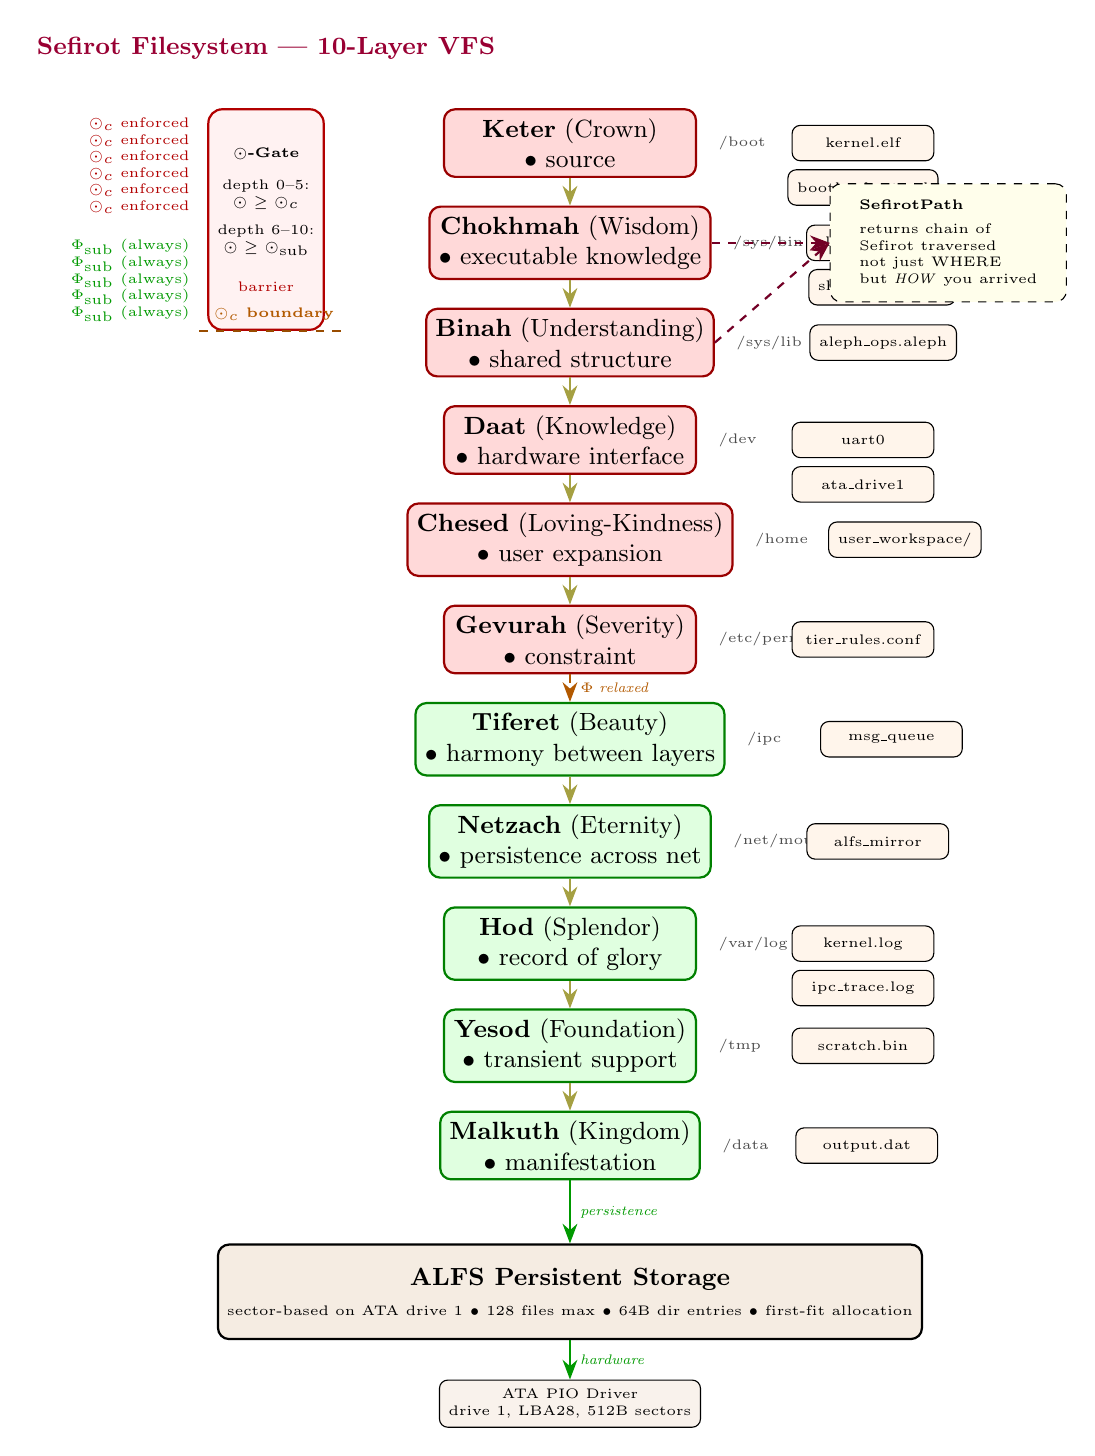
\begin{tikzpicture}[
  node distance=0.4cm and 1.5cm,
  sefirah/.style={rectangle, draw, thick, rounded corners, minimum width=3.2cm, minimum height=0.65cm, align=center, font=\small},
  phi_high/.style={sefirah, fill=red!15, draw=red!60!black},
  phi_low/.style={sefirah, fill=green!12, draw=green!50!black},
  phi_gate/.style={rectangle, draw=red!70!black, thick, rounded corners=5pt, fill=red!5, minimum width=1.4cm, minimum height=2.8cm, align=center, font=\tiny},
  file_node/.style={rectangle, draw, thin, rounded corners=3pt, fill=orange!8, minimum width=1.8cm, minimum height=0.45cm, align=center, font=\tiny},
  arrow/.style={-{Stealth[length=2.5mm]}, thick, yellow!60!black},
  arrow_p/.style={-{Stealth[length=2.5mm]}, thick, purple!60!black},
  arrow_g/.style={-{Stealth[length=2.5mm]}, thick, green!60!black},
  arrow_r/.style={-{Stealth[length=2.5mm]}, thick, red!60!black},
  labeln/.style={font=\tiny\itshape, align=center},
  level label/.style={font=\tiny\bfseries, text=gray!70!black}
]

% ============================================================
% PHI GATE (vertical barrier on left)
% ============================================================
\node[phi_gate] (phig) {\textbf{$\odot$-Gate}\\[0.2cm]
  depth 0--5:\\$\odot \ge \odot_c$\\[0.15cm]
  depth 6--10:\\$\odot \ge \odot_{\text{sub}}$\\[0.3cm]
  \normalfont\color{red!70!black} barrier};

% ============================================================
% SEFIROT TREE — 10 levels
% ============================================================
\node[font=\bfseries\small, text=purple!80!black, above=0.5cm of phig.north, anchor=south] (title) {Sefirot Filesystem — 10-Layer VFS};

% Level 0: Keter
\node[phi_high, right=1.5cm of phig.north east, anchor=north west] (keter) {\textbf{Keter} (Crown)\\$\bullet$ source};
\node[font=\tiny, right=0.15cm of keter.east, anchor=west, text=gray!60!black] (k_path) {/boot};
\node[file_node, right=1.2cm of keter.east] (k_f1) {kernel.elf};
\node[file_node, below=0.1cm of k_f1] (k_f2) {bootloader.toml};

% Level 1: Chokhmah
\node[phi_high, below=0.35cm of keter] (chok) {\textbf{Chokhmah} (Wisdom)\\$\bullet$ executable knowledge};
\node[font=\tiny, right=0.15cm of chok.east, anchor=west, text=gray!60!black] (ch_path) {/sys/bin};
\node[file_node, right=1.2cm of chok.east] (ch_f1) {aleph\_repl.aleph};
\node[file_node, below=0.1cm of ch_f1] (ch_f2) {shell\_cmd.aleph};

% Level 2: Binah
\node[phi_high, below=0.35cm of chok] (binah) {\textbf{Binah} (Understanding)\\$\bullet$ shared structure};
\node[font=\tiny, right=0.15cm of binah.east, anchor=west, text=gray!60!black] (bi_path) {/sys/lib};
\node[file_node, right=1.2cm of binah.east] (bi_f1) {aleph\_ops.aleph};

% Level 3: Daat
\node[phi_high, below=0.35cm of binah] (daat) {\textbf{Daat} (Knowledge)\\$\bullet$ hardware interface};
\node[font=\tiny, right=0.15cm of daat.east, anchor=west, text=gray!60!black] (da_path) {/dev};
\node[file_node, right=1.2cm of daat.east] (da_f1) {uart0};
\node[file_node, below=0.1cm of da_f1] (da_f2) {ata\_drive1};

% Level 4: Chesed
\node[phi_high, below=0.35cm of daat] (ches) {\textbf{Chesed} (Loving-Kindness)\\$\bullet$ user expansion};
\node[font=\tiny, right=0.15cm of ches.east, anchor=west, text=gray!60!black] (ch2_path) {/home};
\node[file_node, right=1.2cm of ches.east] (ch2_f1) {user\_workspace/};

% Level 5: Gevurah
\node[phi_high, below=0.35cm of ches] (gev) {\textbf{Gevurah} (Severity)\\$\bullet$ constraint};
\node[font=\tiny, right=0.15cm of gev.east, anchor=west, text=gray!60!black] (ge_path) {/etc/permissions};
\node[file_node, right=1.2cm of gev.east] (ge_f1) {tier\_rules.conf};

% --- PHI GATE BOUNDARY ---
\draw[dashed, thick, orange!60!black] ($(phig.south west)+(-0.1,0)$) -- ($(phig.south east)+(0.3,0)$)
  node[midway, above, font=\tiny\bfseries, text=orange!70!black] {$\odot_c$ boundary};

% Level 6: Tiferet
\node[phi_low, below=0.35cm of gev] (tif) {\textbf{Tiferet} (Beauty)\\$\bullet$ harmony between layers};
\node[font=\tiny, right=0.15cm of tif.east, anchor=west, text=gray!60!black] (ti_path) {/ipc};
\node[file_node, right=1.2cm of tif.east] (ti_f1) {msg\_queue};

% Level 7: Netzach
\node[phi_low, below=0.35cm of tif] (net) {\textbf{Netzach} (Eternity)\\$\bullet$ persistence across net};
\node[font=\tiny, right=0.15cm of net.east, anchor=west, text=gray!60!black] (ne_path) {/net/mount};
\node[file_node, right=1.2cm of net.east] (ne_f1) {alfs\_mirror};

% Level 8: Hod
\node[phi_low, below=0.35cm of net] (hod) {\textbf{Hod} (Splendor)\\$\bullet$ record of glory};
\node[font=\tiny, right=0.15cm of hod.east, anchor=west, text=gray!60!black] (ho_path) {/var/log};
\node[file_node, right=1.2cm of hod.east] (ho_f1) {kernel.log};
\node[file_node, below=0.1cm of ho_f1] (ho_f2) {ipc\_trace.log};

% Level 9: Yesod
\node[phi_low, below=0.35cm of hod] (yes) {\textbf{Yesod} (Foundation)\\$\bullet$ transient support};
\node[font=\tiny, right=0.15cm of yes.east, anchor=west, text=gray!60!black] (ye_path) {/tmp};
\node[file_node, right=1.2cm of yes.east] (ye_f1) {scratch.bin};

% Level 10: Malkuth
\node[phi_low, below=0.35cm of yes] (mal) {\textbf{Malkuth} (Kingdom)\\$\bullet$ manifestation};
\node[font=\tiny, right=0.15cm of mal.east, anchor=west, text=gray!60!black] (ma_path) {/data};
\node[file_node, right=1.2cm of mal.east] (ma_f1) {output.dat};

% ============================================================
% TREE CONNECTIONS (vertical spine)
% ============================================================
\draw[arrow] (keter) -- (chok);
\draw[arrow] (chok) -- (binah);
\draw[arrow] (binah) -- (daat);
\draw[arrow] (daat) -- (ches);
\draw[arrow] (ches) -- (gev);
\draw[arrow, dashed, orange!70!black] (gev) -- (tif) node[midway, right, font=\tiny\itshape, text=orange!70!black] {$\Phi$ relaxed};
\draw[arrow] (tif) -- (net);
\draw[arrow] (net) -- (hod);
\draw[arrow] (hod) -- (yes);
\draw[arrow] (yes) -- (mal);

% ============================================================
% LEFT SIDE: Phi-Gate annotations per level
% ============================================================
\node[font=\tiny, left=0.1cm of phig.north west, anchor=north east, text=red!70!black, align=right] (phi_ann1) {
  $\odot_c$ enforced\\$\odot_c$ enforced\\$\odot_c$ enforced\\$\odot_c$ enforced\\$\odot_c$ enforced\\$\odot_c$ enforced
};
\node[font=\tiny, left=0.1cm of phig.south west, anchor=south east, text=green!60!black, align=right] (phi_ann2) {
  $\Phi_{\text{sub}}$ (always)\\$\Phi_{\text{sub}}$ (always)\\$\Phi_{\text{sub}}$ (always)\\$\Phi_{\text{sub}}$ (always)\\$\Phi_{\text{sub}}$ (always)
};

% ============================================================
% BOTTOM: ALFS Persistence Layer
% ============================================================
\node[rectangle, draw, thick, rounded corners, fill=brown!15, minimum width=8cm, minimum height=1.2cm,
      below=0.8cm of mal, align=center, font=\small] (alfs) {\textbf{ALFS Persistent Storage}\\
  \normalfont\tiny sector-based on ATA drive 1 $\bullet$ 128 files max $\bullet$ 64B dir entries $\bullet$ first-fit allocation};

\node[rectangle, draw, thin, rounded corners=3pt, fill=brown!10, minimum width=2cm, minimum height=0.45cm,
      below=0.5cm of alfs, align=center, font=\tiny] (ata) {ATA PIO Driver\\drive 1, LBA28, 512B sectors};

\draw[arrow_g] (mal.south) -- (alfs.north) node[midway, right, labeln] {persistence};
\draw[arrow_g] (alfs.south) -- (ata.north) node[midway, right, labeln] {hardware};

% ============================================================
% TOP RIGHT: SefirotPath annotation
% ============================================================
\node[rectangle, draw, dashed, rounded corners, fill=yellow!8, minimum width=3cm, minimum height=1.5cm,
      right=1.5cm of chok.east, align=left, font=\tiny] (spath) {
  \textbf{SefirotPath}\\[0.1cm]
  \normalfont returns chain of\\Sefirot traversed\\not just WHERE\\but \emph{HOW} you arrived
};

\draw[arrow_p, dashed] (chok.east) -- (spath.west);
\draw[arrow_p, dashed] (binah.east) -- (spath.west);

% ============================================================
% TITLE
% ============================================================

\end{tikzpicture}
\end{document}
